\section{L�sen von SAT-Problemen mit SAT-Solver}

SAT-Probleme bedeuten boolesche Erf�llbarkeitsprobleme. Solche Probleme k�nnen mit einem SAT-Solver gel�st werde. Dies kann erfolgen, indem einfach boolesche Formeln \(\phi\) an einen SAT-Solver �bergeben werden, der dann nach \(I(\phi)=TRUE\) aufl�st.

\begin{figure}[H]
    \centering
    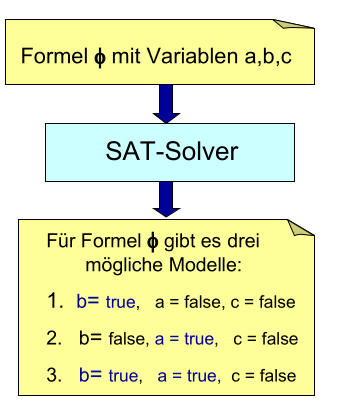
\includegraphics[width=0.4\textwidth]{figures/kap8/SAT-solver.png}
    \caption{Verwendung eines SAT-Solvers}
    \label{fig:using-sat-solver}
\end{figure}

Abbildung~\ref{fig:using-sat-solver} zeigt die Ausgabe der Variablen a,b,c mit der folgenden Formel:

\[ \phi = (a \vee b \vee c) \wedge (a \Rightarrow \neg(a \wedge c)) \wedge (c \Rightarrow (a \wedge c \vee b \wedge c)) \wedge (\neg a \Rightarrow (\neg c \wedge b \vee \neg b \wedge c))\]

Was die folgende Wahrheitstabelle ergibt:

\begin{figure}[H]
    \centering
    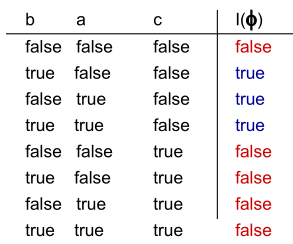
\includegraphics[width=0.4\textwidth]{figures/kap8/truth-table-SAT.png}
    \caption{Wahrheitstabelle des SAT-Problems}
    \label{fig:sat-solver-truthtable}
\end{figure}

Ein Beispiel f�r eine Anwendung eines SAT Solvers ist das Spiel Sudoku. Man kann die Einschr�nkungen der Sudoku-Felder mit einer Logiksprache definieren und dann einen SAT-Solver verwenden, um ein Modell zu finden, das das Problem l�sen kann.